
\includegraphics[height=1.5cm]{images/pictograms/benchmark}

\lstinputlisting[language=bash,basicstyle=\small]{python_codes/fieldstone_76/keywords.ascii}

\begin{center}
Code at \url{https://github.com/cedrict/fieldstone/tree/master/python_codes/fieldstone_76}
\end{center}

\par\noindent\rule{\textwidth}{0.4pt}

%%%%%%%%%%%%%%%%%%%%%%%%%%%%%%%%%%%%%%%%%%%%%%%%%%%%%%%%%%%%%%%%%%%%%%%%%%%%%%%%%%%%%%%%%%%%


This stone is an example of $Q_2\times P_{-1}$ implementation. 
The 2D $Q_2$ shape functions have been derived in Section~\ref{MMM-ss:q22d}
The $-1$ subscript indicates that the pressure field is linear (but not bilinear!).

Actually the story is a bit more complicated than that, as explained for 
example in \textcite{boga02} (2002):
``Two possible choices are given for the definition of the pressure space: 
one can either use a global pressure approximation (that is on
each quadrilateral the finite element space is spanned by 1 and by the global co-ordinates $x$ and $y$)
or a local approach (consisting in generating the local space by means of the constants and the local
curvilinear co-ordinates on each quadrilateral $r$ and $s$). [...] Numerical results actually show
that the second choice (local or mapped pressure approximation) is suboptimally convergent.'' 

In other words, the mapped version consists of  
using the $P_{-1}$ basis functions defined in Section~\ref{MMM-ss:lbfq2D}:
inside the element the pressure is given by $p^h(r,s)=a+br+cs$ 

The unmapped version is a bit less straightforward and is as follows:
let us assume there are three pressure nodes inside the element.
Inside the element, the pressure is defined by a linear field
\[
p^h(x,y) = a+bx+cy
\]
We must then compute the coefficients $a,b,c$. We know that 
the expression above evaluated at the pressure nodes with coordinates $(x_i,y_i)$ should 
be equal to $p_i$. Then we have the following three equations:
\begin{eqnarray}
a + bx_1 + cy_1 &=& p_1 \nn\\
a + bx_2 + cy_2 &=& p_2 \nn\\
a + bx_3 + cy_3 &=& p_3 \nn
\end{eqnarray}
or, 
\[
\left(
\begin{array}{ccc}
1 & x_1 & y_1 \\
1 & x_2 & y_2 \\
1 & x_3 & y_3 
\end{array}
\right)
\cdot 
\left(
\begin{array}{ccc}
a \\ b \\ c
\end{array}
\right)
=
\left(
\begin{array}{ccc}
p_1 \\ p_2 \\ p_3
\end{array}
\right)
\]
Then 
\[
\left(
\begin{array}{ccc}
a \\ b \\ c
\end{array}
\right)
=
\left(
\begin{array}{ccc}
1 & x_1 & y_1 \\
1 & x_2 & y_2 \\
1 & x_3 & y_3 
\end{array}
\right)^{-1}
\cdot
\left(
\begin{array}{ccc}
p_1 \\ p_2 \\ p_3
\end{array}
\right)
= {\bm M}^{-1} \cdot \vec{p}
\]
with 
\[
\Delta = x_2y_3-x_3y_2 - x_1y_3-x_3y_1 + x_1y_2-x_2y_1
\]
and 
\[
{\bm M}^{-1} = \frac{1}{\Delta}
\left(
\begin{array}{ccc}
x_2y_3-x_3y_2 & x_3y_1-x_1y_3 & x_1y_2-x_2y_1 \\
y_2-y_3 & y_3-y_1 & y_1-y_2 \\
x_3-x_2 & x_1-x_3 & x_2-x_1
\end{array}
\right)
=
\left(
\begin{array}{ccc}
m_{11} & m_{12} & m_{13} \\
m_{21} & m_{22} & m_{23} \\
m_{31} & m_{32} & m_{33} 
\end{array}
\right)
\]
\begin{eqnarray}
a &=& m_{11}p_1 + m_{12} p_2 + m_{13} p_3 \nn\\
b &=& m_{21}p_1 + m_{22} p_2 + m_{23} p_3 \nn\\
c &=& m_{31}p_1 + m_{32} p_2 + m_{33} p_3 \nn
\end{eqnarray}
so 
\begin{eqnarray}
p^h(x,y) 
&=&  a+bx+cy \nn\\
&=& m_{11}p_1 + m_{12} p_2 + m_{13} p_3
+ (m_{21}p_1 + m_{22} p_2 + m_{23} p_3) x
+ (m_{31}p_1 + m_{32} p_2 + m_{33} p_3) y \nn\\
&=& \underbrace{(m_{11} + m_{21}x + m_{31}y)}_{N_1(x,y)} p_1 
+   \underbrace{(m_{12} + m_{22}x + m_{32}y)}_{N_2(x,y)} p_2 
+   \underbrace{(m_{13} + m_{23}x + m_{33}y)}_{N_3(x,y)} p_3
\end{eqnarray}
The basis functions are then evaluated at the (real) coordinates 
of the quadrature point $(x_q,y_q)$.

Note that I use isoparametric elements where the $Q_2$ basis 
functions are used for the mapping. In the case of 
rectangular elements the approaches above (mapped and unmapped)
yield the same pressure basis functions values at the quadrature points
so the measured errors and vrms are identical. 


In both cases the pressure is discontinuous from an element to another and
this poses a little problem in terms of exporting it to vtu (and plotting with paraview).
I then simply choose to export the value of the pressure in the middle of 
each element. 

When mesh randomization is added to all nodes, I make sure that the velocity 
nodes 4,5,6,7 in the middle of the edges 
are really put back between nodes 0-1, 1-2, 2-3, and 3-0 respectively. The node in the middle of the element
is also then moved accordingly. 

I also explore the effect of the number of quadrature points on the solution, 
so I allow for $2^2$, $3^2$ and $4^2$ quadrature points. 

I carry out three benchmarks based on manufactured solutions  
and recover the expected cubic convergence for the velocity error 
and a quadratic error convergence for the pressure \textit{only} for the unmapped approach
in the case of non-rectangular elements.



%.......................................................
\subsection*{Manufactured solution of Donea \& Huerta ({\tt bench=3})}

This is the Donea \& Huerta benchmark, see Section~\ref{MMM-mms1}.

\begin{center}
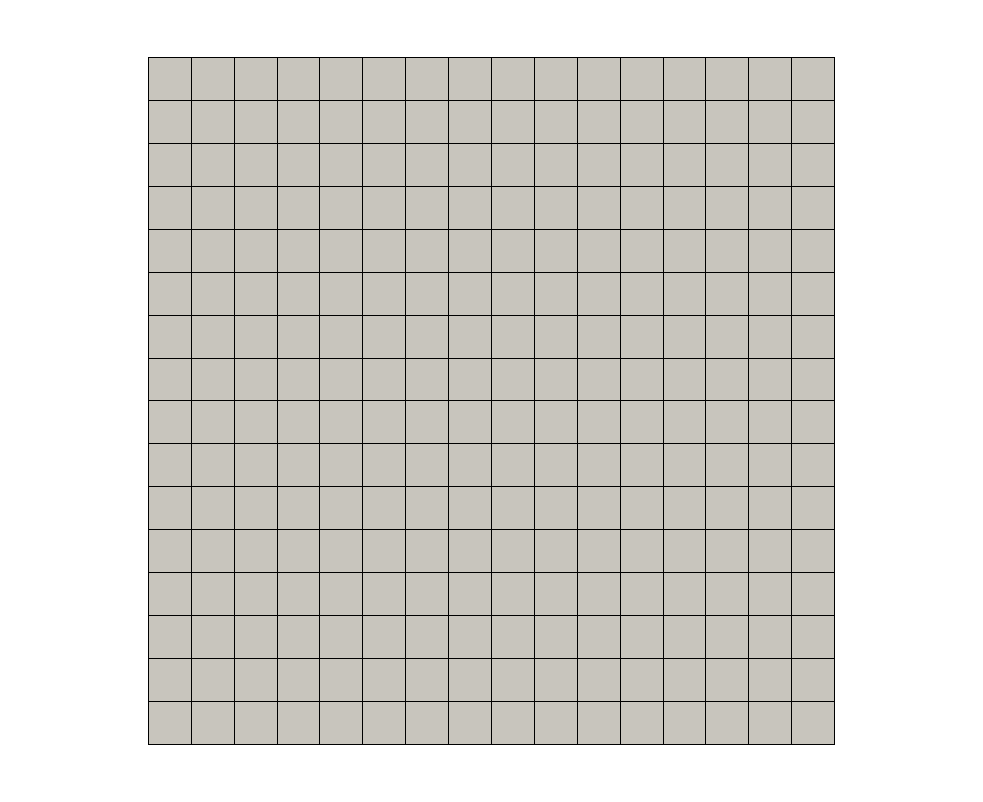
\includegraphics[width=6cm]{python_codes/fieldstone_76/results/dh/reg/mesh_reg}
\includegraphics[width=8cm]{python_codes/fieldstone_76/results/dh/reg/vrms}\\
\includegraphics[width=8cm]{python_codes/fieldstone_76/results/dh/reg/errors_V}
\includegraphics[width=8cm]{python_codes/fieldstone_76/results/dh/reg/errors_P}\\
{\captionfont Regular square mesh}
\end{center}

\begin{center}
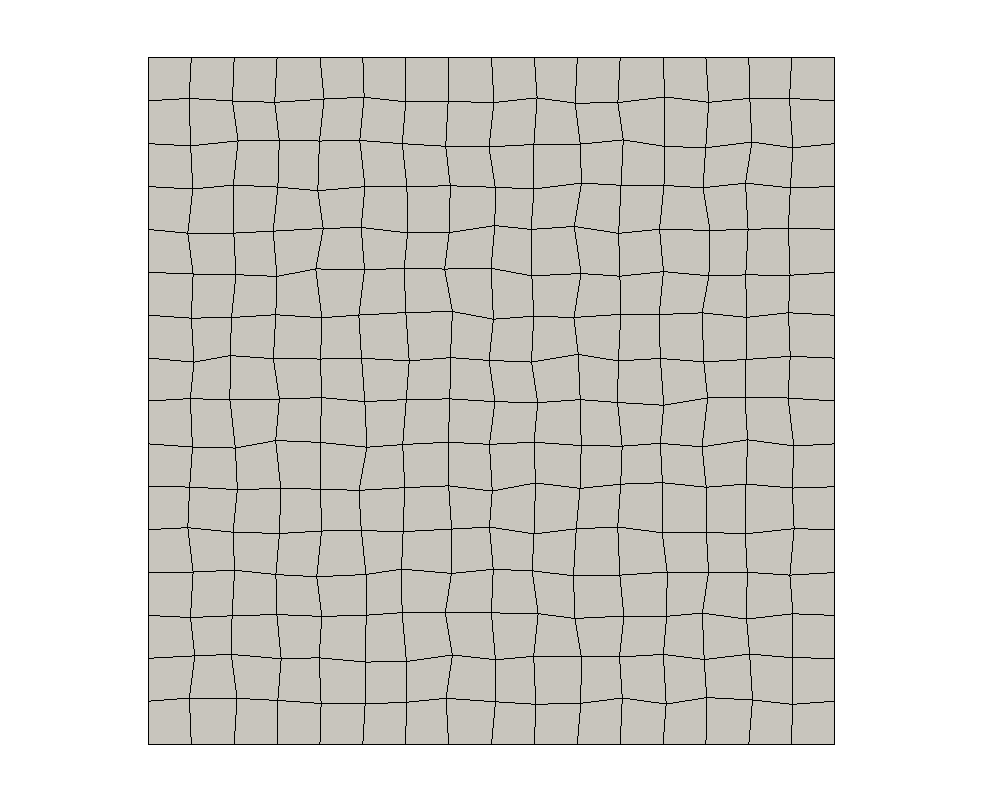
\includegraphics[width=6cm]{python_codes/fieldstone_76/results/dh/rand/mesh_rand}
\includegraphics[width=8cm]{python_codes/fieldstone_76/results/dh/rand/vrms}\\
\includegraphics[width=8cm]{python_codes/fieldstone_76/results/dh/rand/errors_V}
\includegraphics[width=8cm]{python_codes/fieldstone_76/results/dh/rand/errors_P}\\
{\captionfont Randomized $\xi=0.1$ mesh}
\end{center}

The observed super-convergence of the pressure for $n_q=2^2$ is probably due to the 
pressure field being too 'simple' in this case.

%......................................................
\subsection*{Manufactured solution \#1 ({\tt bench=1})}

The analytical solution originates in Lamichhane (2017) \cite{lami17}.
The velocity and pressure are given by
\begin{eqnarray}
u(x,y)&=&-2x^2y(2y-1)(x-1)^2(y-1) \\
v(x,y)&=& 2xy^2(2x-1)(x-1)(y-1)^2 \\
p(x,y)&=& x(1-x)(1-2y)
\end{eqnarray}
Boundary conditions are no-slip on all sides of the unit square. 
The corresponding body force terms are derived in Section~\ref{MMM-ss:mms11}. 

\begin{center}
\includegraphics[width=5.7cm]{python_codes/fieldstone_76/results/mms1/reg/vrms}
\includegraphics[width=5.7cm]{python_codes/fieldstone_76/results/mms1/reg/errors_V}
\includegraphics[width=5.7cm]{python_codes/fieldstone_76/results/mms1/reg/errors_P}\\
{\captionfont Regular square mesh}
\end{center}

\begin{center}
\includegraphics[width=5.7cm]{python_codes/fieldstone_76/results/mms1/rand/vrms}
\includegraphics[width=5.7cm]{python_codes/fieldstone_76/results/mms1/rand/errors_V}
\includegraphics[width=5.7cm]{python_codes/fieldstone_76/results/mms1/rand/errors_P}\\
{\captionfont Randomized $\xi=0.1$ mesh}
\end{center}

%......................................................
\subsection*{Manufactured solution \#2 ({\tt bench=9})}

This is the second manufactured solution 
mentioned in Lamichhane \cite{lami17}. It is presented in Section~\ref{MMM-ss:mms2}.
It is for a unit square with $\eta=1$ and the smooth exact solution is
\begin{eqnarray}
u(x,y) &=& x+x^2 - 2xy+x^3 - 3xy^2 + x^2y \\
v(x,y) &=& -y-2xy+y^2 -3x^2y + y^3 - xy^2 \\
p(x,y) &=& xy+x+y+x^3y^2 - 4/3
\end{eqnarray}
Note that the pressure obeys $\int_{\Omega} p \; dV = 0$. The analytical 
velocity is prescribed on the boundary of the domain. 

\begin{center}
\includegraphics[width=5.7cm]{python_codes/fieldstone_76/results/mms2/reg/vrms}
\includegraphics[width=5.7cm]{python_codes/fieldstone_76/results/mms2/reg/errors_V}
\includegraphics[width=5.7cm]{python_codes/fieldstone_76/results/mms2/reg/errors_P}\\
{\captionfont Regular square mesh}
\end{center}

\begin{center}
\includegraphics[width=5.7cm]{python_codes/fieldstone_76/results/mms2/rand/vrms}
\includegraphics[width=5.7cm]{python_codes/fieldstone_76/results/mms2/rand/errors_V}
\includegraphics[width=5.7cm]{python_codes/fieldstone_76/results/mms2/rand/errors_P}\\
{\captionfont Randomized $\xi=0.1$ mesh}
\end{center}


%.......................................................
\subsection*{Instantaneous sinking block}

It is fully described in Section~\ref{MMM-ss:sinking_block}

\begin{center}
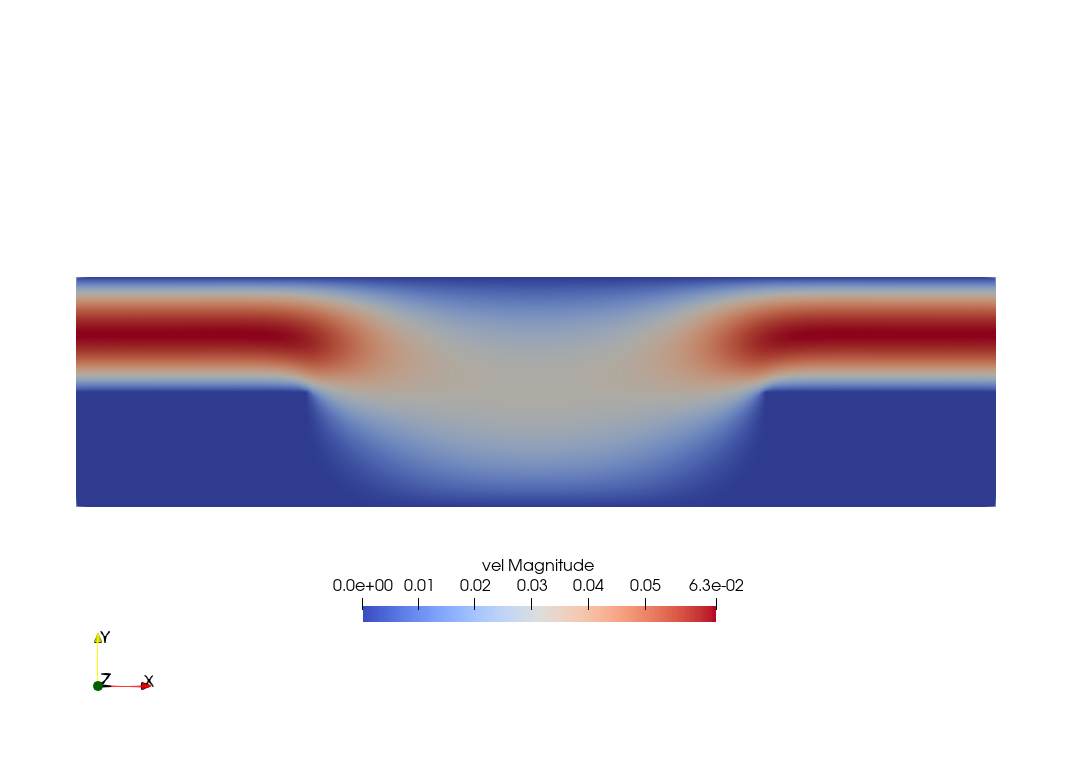
\includegraphics[width=7cm]{python_codes/fieldstone_76/results/block/vel}
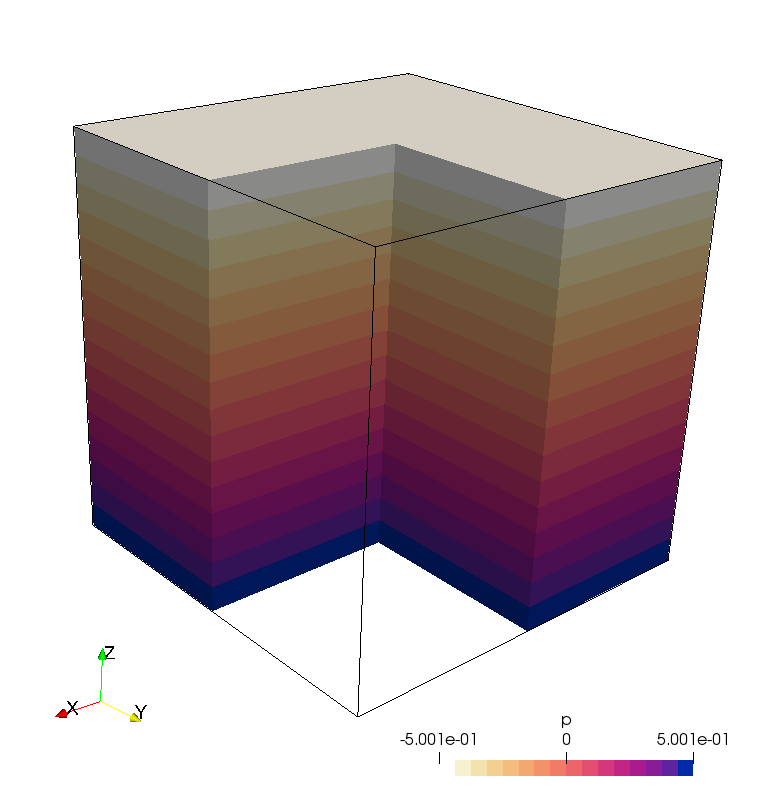
\includegraphics[width=7cm]{python_codes/fieldstone_76/results/block/press}
\end{center}


